\chapter{Conceptual Design}

\subsection{Requirements}

\begin{table}[H]
    \renewcommand{\arraystretch}{1.25}
    \begin{tabularx}{\textwidth}{|X|}
    \hline
    \multicolumn{1}{|c|}{\textbf{``StageUp Inc.''}} \\
    \hline
    The company ``StageUp'' has a central office and several operational depots located across the world, each covering a specific region, which consists of one or more municipalities, where they manage the rental and installation of audiovisual equipment for events. The central office does not handle physical setups. Both the central office and depots are characterized by name, address, city/province, and number of employees. Bookings, either recurring or one-time, are coordinated by the central office. Bookings can be placed by customers via phone, postal mail, email, or through the website. Besides one-time bookings, the company also handles seasonal contracts and special promotional rentals. Bookings are delivered and installed at customer event locations, which are characterized by address, house number, postal code, city, and province. Since each customer can have one or more event locations, each address is identified by a unique code within the customer's profile. Additionally, each event location has a setup time estimate and equipment capacity. Depots have one or more setup teams, each with a maximum number of members. Each team is characterized by an identification code, a name, the number of installations made, and some personal data of its team members. Each booking is characterized by type, date, duration, cost, the team that handled it, and the details of the customer who placed it. Customers, classified as individuals or companies, are identified by an alphanumeric code and their personal details. \\
    \hline
    \end{tabularx}
    \caption{Requirements text}
\end{table}

\subsection{Analysis}

\subsubsection{Reorganization of Concepts}

The concepts can be reorganized as follows:

\begin{table}[H]
    \renewcommand{\arraystretch}{1.25}
    \begin{tabularx}{\textwidth}{|X|}
    \hline
    \multicolumn{1}{|c|}{\textbf{Depot}} \\
    \hline
    StageUp operates several operational depots distributed worldwide. Each depot covers a specific region composed of one or more municipalities, is described by name, address, city/province and number of employees, and organizes one or more setup teams that perform installations. \\
    \hline
    \end{tabularx}
    \caption{Depot's Concepts}
\end{table}

\begin{table}[H]
    \renewcommand{\arraystretch}{1.25}
    \begin{tabularx}{\textwidth}{|X|}
    \hline
    \multicolumn{1}{|c|}{\textbf{Setup Team}} \\
    \hline
    Each depot has one or more setup teams. A setup team is characterized by an identification code, a name, the number of installations made, a maximum number of members, and personal information related to its team members. \\
    \hline
    \end{tabularx}
    \caption{Setup Team's Concepts}
\end{table}

\begin{table}[H]
    \renewcommand{\arraystretch}{1.25}
    \begin{tabularx}{\textwidth}{|X|}
    \hline
    \multicolumn{1}{|c|}{\textbf{Booking}} \\
    \hline
    Bookings are coordinated by the central office and can be recurring or one-time. They can be placed by customers through different channels (phone, postal mail, email, website), and include seasonal contracts and special promotional rentals. Each booking is described by type, date, duration, cost, and by the setup team that handled the service. \\
    \hline
    \end{tabularx}
    \caption{Booking's Concepts}
\end{table}

\begin{table}[H]
    \renewcommand{\arraystretch}{1.25}
    \begin{tabularx}{\textwidth}{|X|}
    \hline
    \multicolumn{1}{|c|}{\textbf{Customer}} \\
    \hline
    Customers place bookings and are classified as individuals or companies. They are identified by an alphanumeric code and their personal details, and each customer can manage one or more event locations where installations are performed. \\
    \hline
    \end{tabularx}
    \caption{Customer's Concepts}
\end{table}

\begin{table}[H]
    \renewcommand{\arraystretch}{1.25}
    \begin{tabularx}{\textwidth}{|X|}
    \hline
    \multicolumn{1}{|c|}{\textbf{Event Location}} \\
    \hline
    Event locations are the places where bookings are delivered and installed. Each location is characterized by address, house number, postal code, city and province; within each customer's profile, every location is identified by a unique code. An event location also stores setup time estimate and equipment capacity. \\
    \hline
    \end{tabularx}
    \caption{Event Location's Concepts}
\end{table}

\subsubsection{Glossary of Terms}

\begin{table}[H]
    \renewcommand{\arraystretch}{1.25}
    \begin{tabularx}{\textwidth}{|X|X|X|X|}
    \hline
    \textbf{Term} & \textbf{Description} & \textbf{Connections} & \textbf{Synonyms} \\
    \hline
    Depot & A StageUp Inc. depot. & Setup Team & Region \\
    \hline
    Setup Team & A team that handles rental and installation. & Depot, Booking & Team \\
    \hline
    Booking & A specific booking placed by a customer on the StageUp Inc. platform. & Customer, Event Location, Setup Team & Rental, Contract \\
    \hline
    Customer & User of the StageUp Inc. platform. & Booking, Event Location & \\
    \hline
    Event Location & One of the different locations of a customer. & Customer, Booking & Address \\
    \hline
    \end{tabularx}
    \caption{Glossary of Terms}
\end{table}

\subsubsection{Level of Abstraction}

At the conceptual level, the term \textbf{Region} is absorbed into \textbf{Depot}. This choice is directly motivated by the track sentence: \emph{``each covering a specific region, which consists of one or more municipalities''}. In this context, region does not introduce an autonomous business object with its own independent lifecycle, but identifies the coverage area of exactly one depot. Therefore, in the conceptual schema, \textbf{Depot} and \textbf{Region} are treated as a single abstraction.

The mention of municipalities is consistent with this decision: municipalities describe the internal composition of the covered region, not an additional core entity required by the current conceptual scope. For this reason, the model keeps \textbf{Depot} as the only main term at this level and postpones detailed territorial representation to the complete ER specification, where needed.

The same abstraction criterion is applied to \textbf{Central Office}. Although explicitly mentioned in the track, central office refers to a single organizational instance of StageUp Inc. and does not represent a plural, independent entity to be managed as a central part of the data model. Since the database is built for StageUp operations and the central office has no operational setup role, introducing a dedicated entity for it would add complexity without modeling benefit. Consequently, Central Office is not included as a standalone entity in the skeleton schema and is treated only as organizational context.

\subsubsection{Entity-Relationship Diagram}

\paragraph{SKELETON SCHEMA} \leavevmode \newline
\begin{figure}[H]
    \centering
    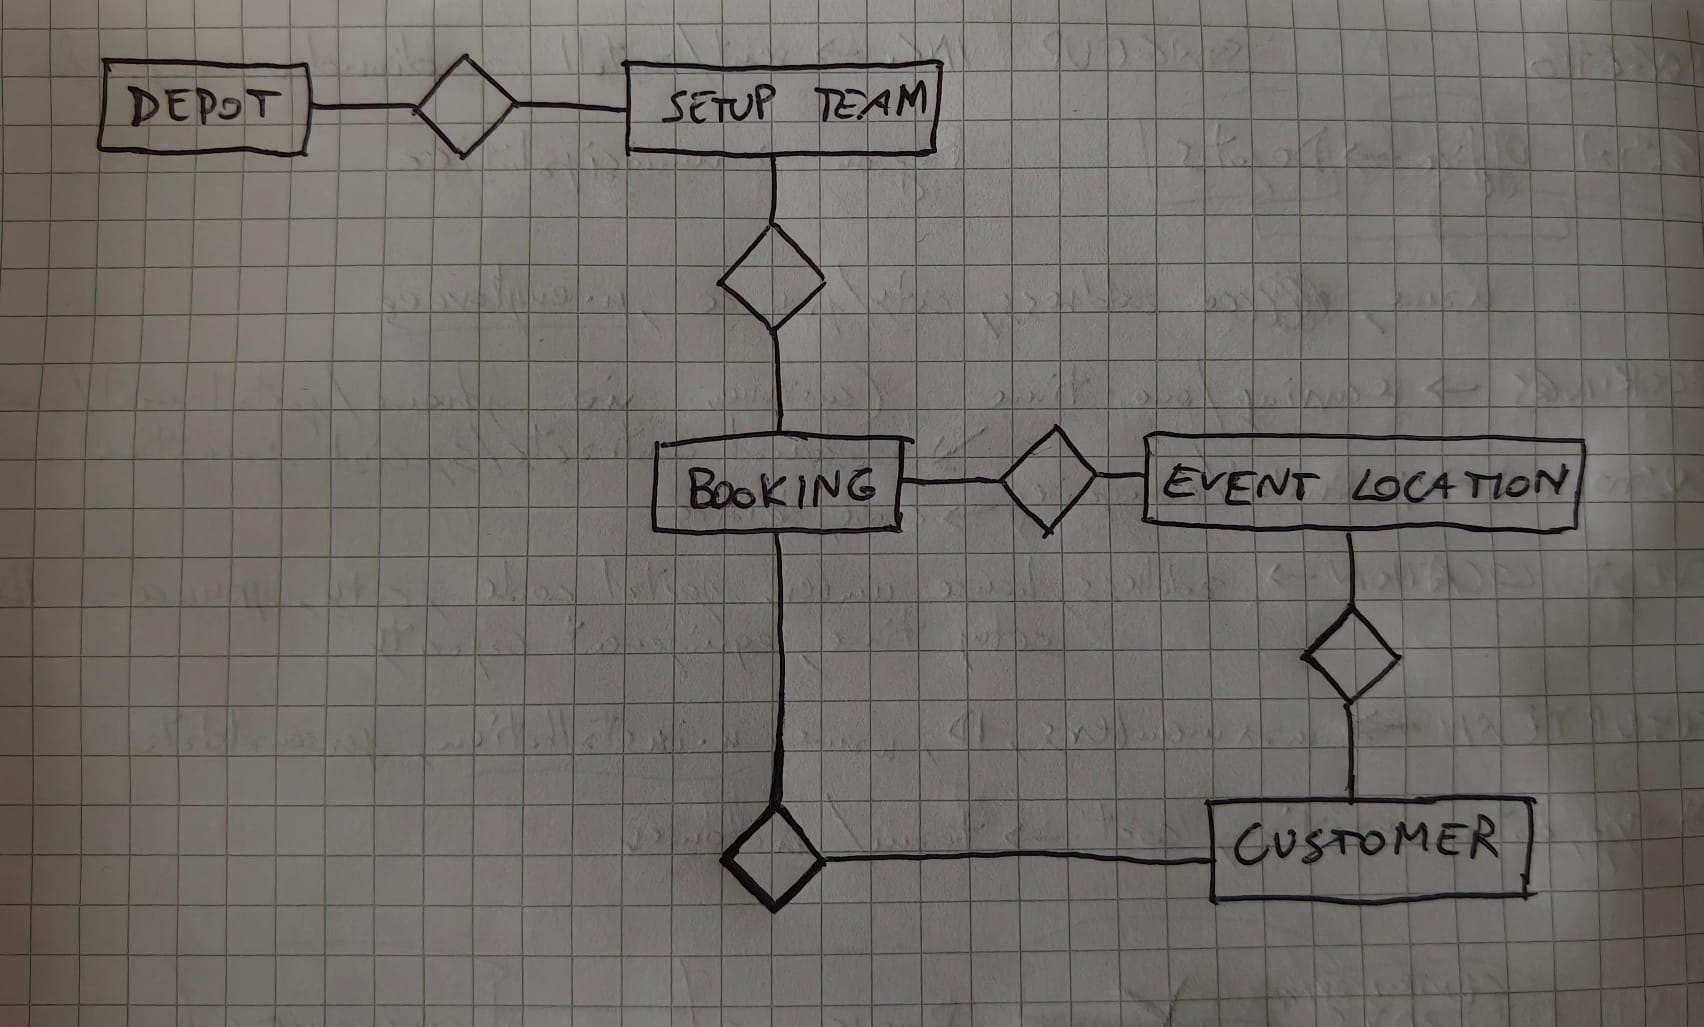
\includegraphics[width=\textwidth]{images/skeleton.jpeg}
    \caption{Skeleton Schema}
\end{figure}

\paragraph{FINAL SCHEMA} \leavevmode \newline
\begin{figure}[H]
    \centering
    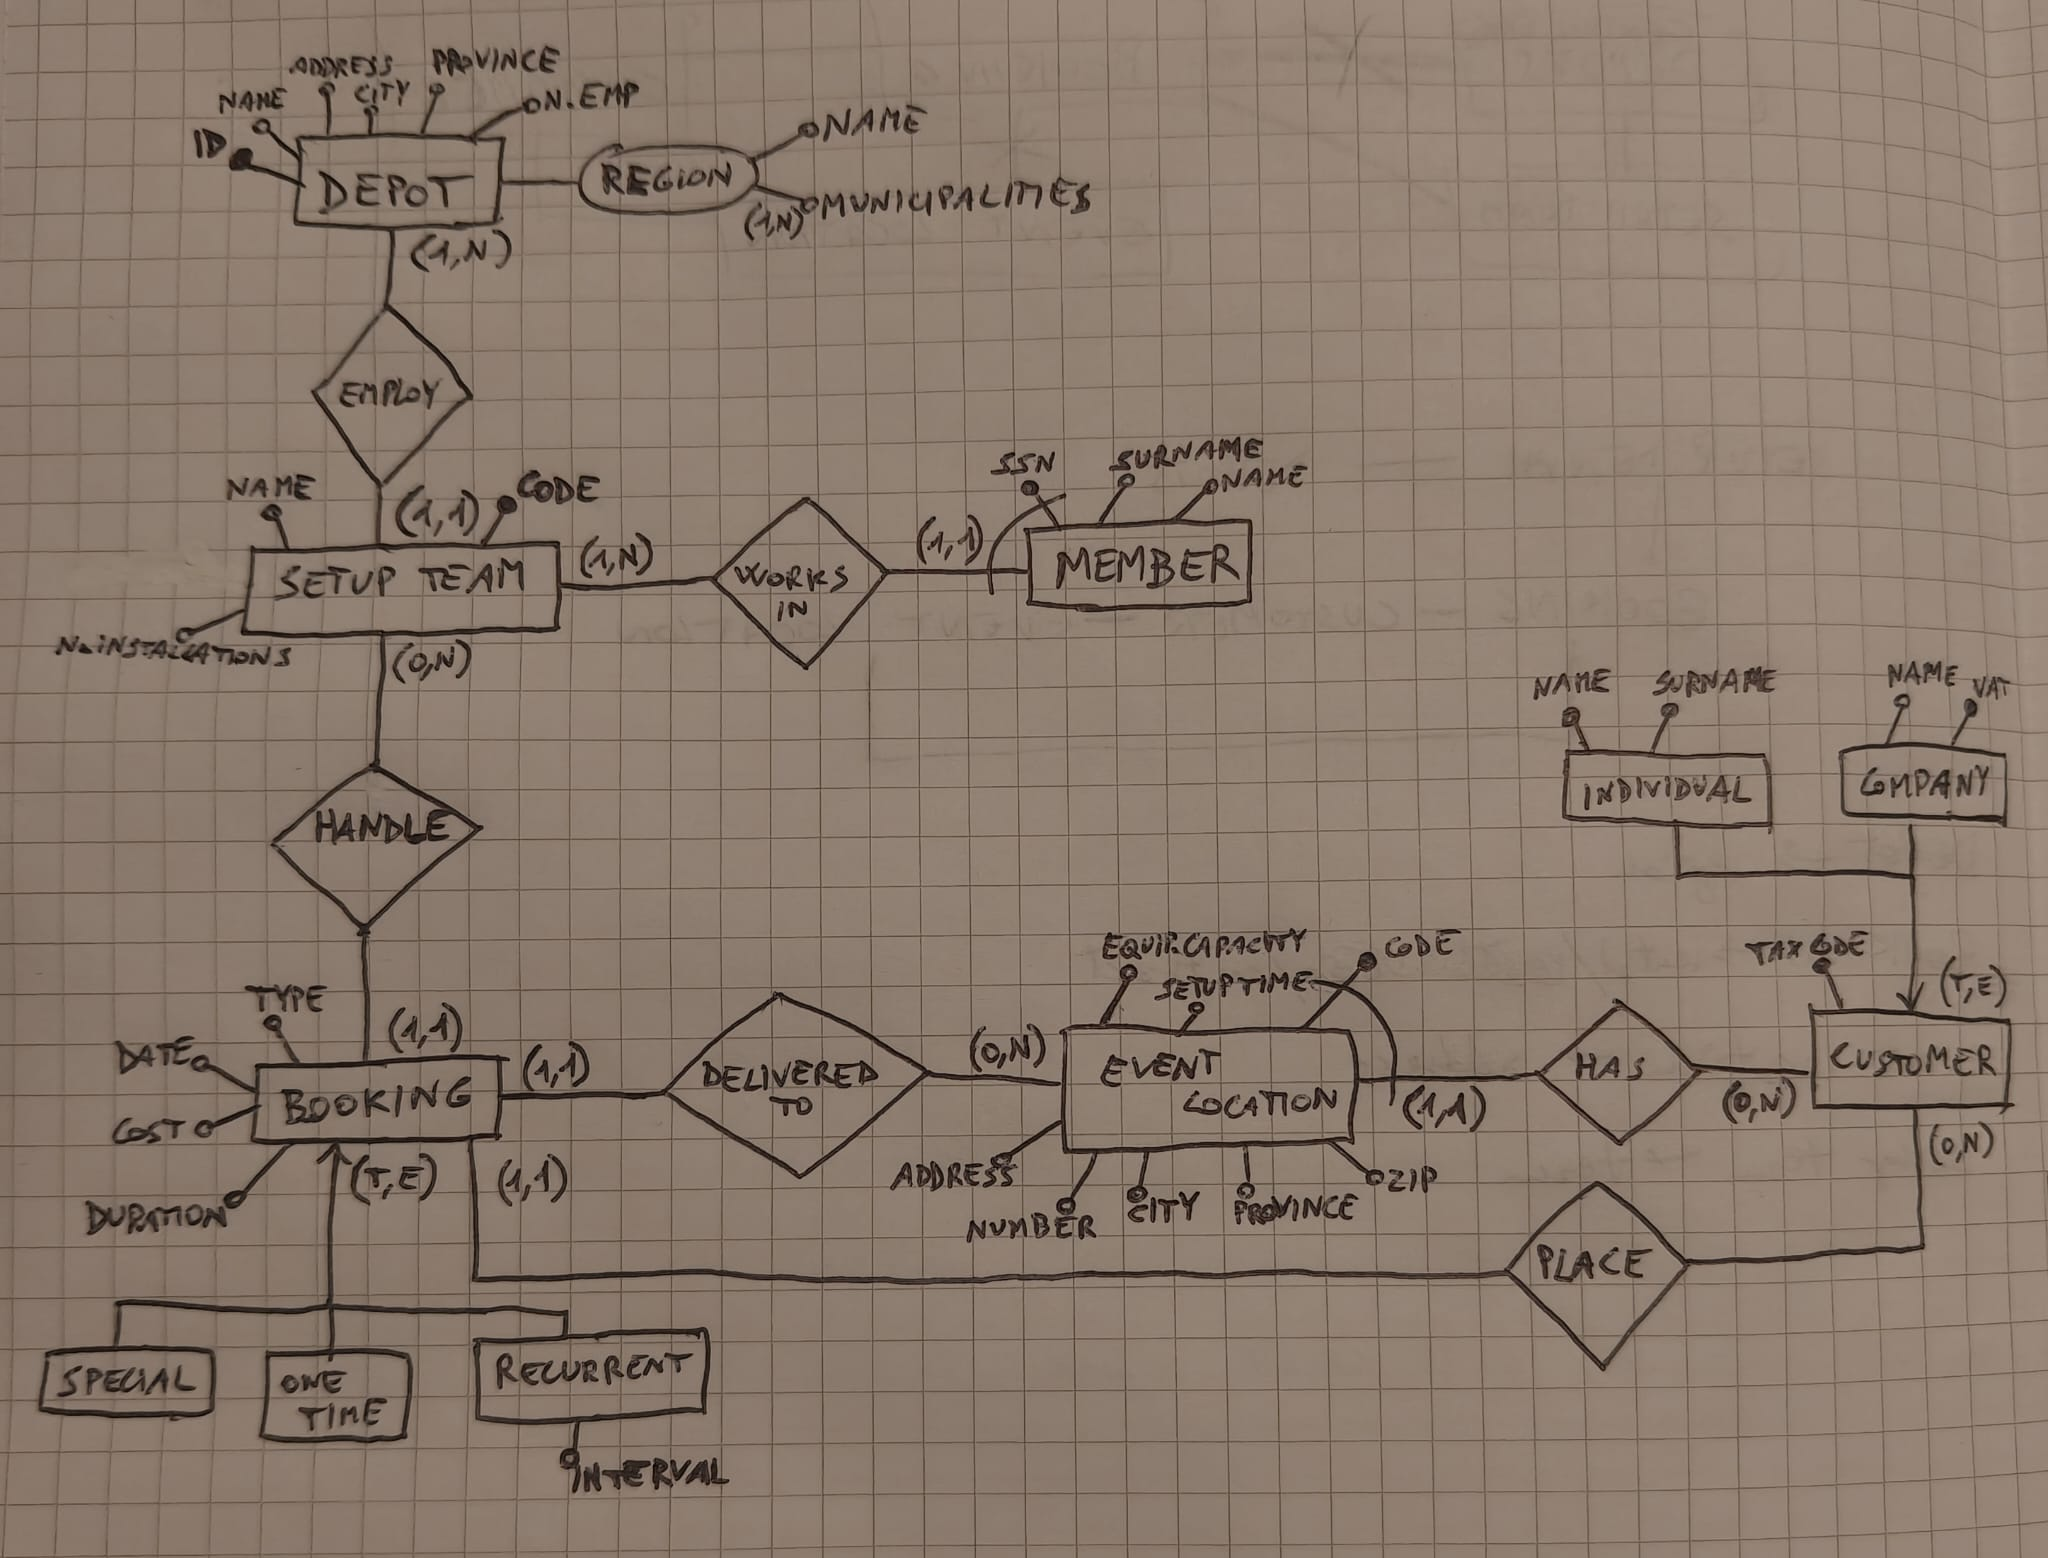
\includegraphics[width=\textwidth]{images/ER FINAL.jpeg}
    \caption{Final Schema}
\end{figure}

\noindent In this final ER schema, \textbf{Region} is not modeled as an autonomous entity; it is represented as a \textbf{composite attribute} of \textbf{Depot}, where \textbf{municipalities} is a \textbf{multivalued attribute}. This modeling choice is consistent with the requirements, since Region does not introduce additional standalone attributes beyond territorial composition. The association between \textbf{Depot} and \textbf{Region} is therefore treated as \textbf{1:1}.

\noindent Conversely, \textbf{Member} is modeled as a proper \textbf{entity}, because the requirements explicitly include personal data (e.g., SSN, name, surname), which should be represented explicitly in the conceptual model. In relation to \textbf{Setup Team}, the cardinality is \textbf{1:N}.

\noindent The attribute \textbf{Max members} has been removed from the \textbf{Setup Team} entity in the ER model, since the track explicitly states that each team may contain at most \textbf{10 members}. For this reason, the limit is treated as a fixed business constraint rather than as a stored attribute.

\subsubsection{Business Rules}
The business rules are the following:
\begin{itemize}
    \item Booking type must be one of \textbf{Phone (P)}, \textbf{Mail (M)}, \textbf{Website (W)}, or \textbf{Email (E)}.
    \item The number of installations of each \textbf{Setup Team} is updated automatically.
    \item A \textbf{Setup Team} can be composed of at most \textbf{10 members}.
    \item A \textbf{Special Booking} is created automatically for the customer and is not placed directly by the customer.
    \item A \textbf{Seasonal Contract} is a \textbf{Recurrent Booking} with a fixed interval of \textbf{4 months}.
\end{itemize}
